
\subsubsection{HDL Neural Network}

A number of modules has been implemented to achieve fully functional neural network:
\begin{itemize}
    \item 32Bit floating point compare unit (greater than, greater equal, less than, less equal)
    \item Cascade adder
    \item Neural module
    \item Layer module
    \item ReLu activation
    \item Hard Sigmoid activation
\end{itemize}

Number of modules have been combined together to test $8 \times 8 \times 2$ network that was trained for 2bit IQ modulation (resulting with modulation that looks similar to 4QAM). Internal neural state was identical to one in simulation, output was slightly different due to hard sigmoid function being used instead of regular sigmoid.


\begin{figure}[H]
    \centering
    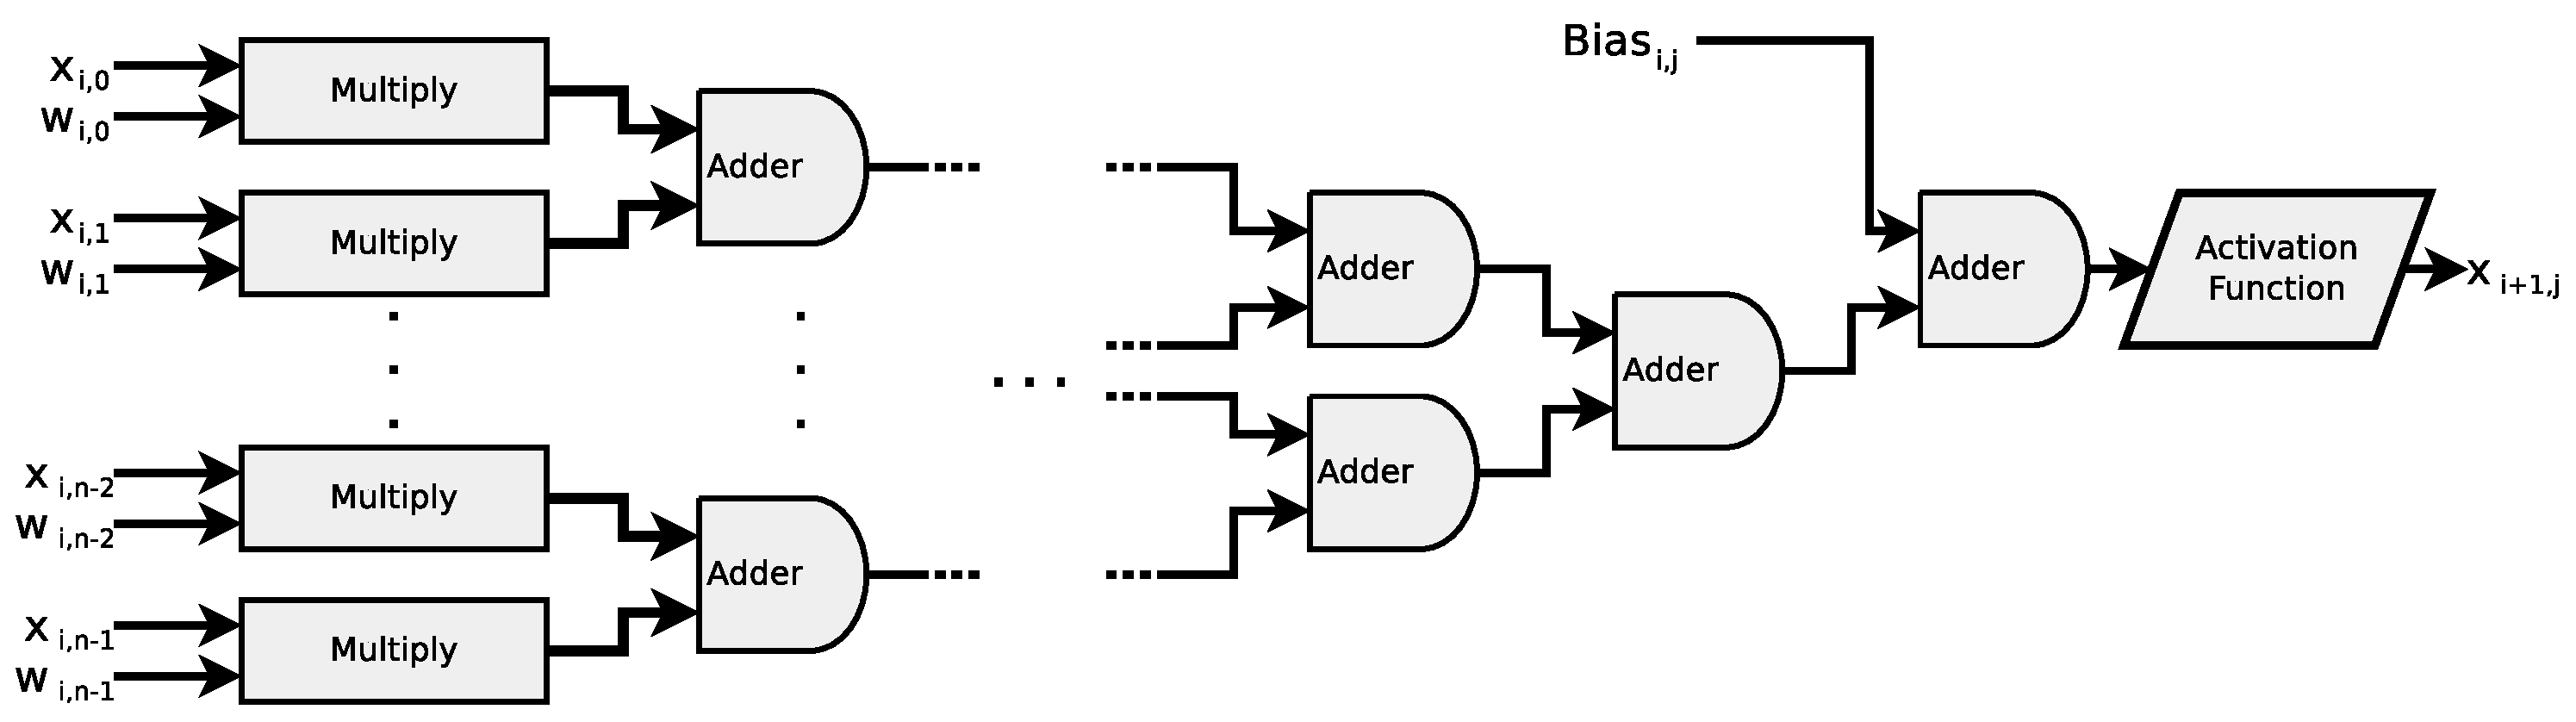
\includegraphics[width=1.05\linewidth]{digital_circ/neuron.eps}
    \caption{Single Digital Neuron Circuit where x is other neuron connection, w - weight, i - layer number, j - neuron number, n - number of neurons in layer.}
    \label{fig:neuron_circ}
\end{figure}

\subsubsection{Cascade Adder}
Cascade adder was the most complex part of the design as module needed to be parameterised. At this point only $2^N$ input signals are considered. Many complications from the fact that this is a dynamically generated module that is not proportional in size - that is 8 input adder would have 3 stages, first having 4 adders, second 2 and last 1. After multiple attempts I concluded that it is impossible to implement this module using conventional loop programming because there is no way set previous and next connections in a single stage as a variable and reuse it in each for loop. Two other solutions were implemented:

\begin{enumerate}
  \item Create a 2D unpacked matrix that contain all connections - this matrix would be $2^{N-1}$ height and $N-1$ width where N is number of stages. Only down side to this solution is that only half of matrix would be always populated because each stage requires twice as many connections. This might not be a problem with a small cascades. HDL synthesizer might optimise such matrix but this needs to be confirmed.
  \item Create a 1D array of connections and calculate indexes of correct connection in each for loop stage. This method required to solve some simple geometric series in order to find index of first connection of each stage at the start of for loop which is shown in \autoref{eq:sum}.
\end{enumerate}

\begin{equation}\label{eq:sum}
    S_n = \sum_{n=0}^m 2^{K-2-n} = 2^{K-2}\frac{2^m-1}{2^m}
\end{equation}
Where K in total number of stages, m is stage.


\subsubsection{Floating Point Arithmetic}

Open source 32 bit floating point arithmetic modules written with SystemVerilog has been adopted to implement neural network. This modules been used for addition and multiplication. It however had three negative sides:
\begin{enumerate}
  \item It uses Synchronous Interconnect Bus shown in \autoref{fig:abus}. When module A is ready to send data, it sends data, sets \textit{stb} (strobe) flat high and freezes until \textit{ack} (acknowledgment) flag is set high by module B indicating that data was accepted. This allows synchronous module communication when each module takes unknown amount of time to compute its input, however downside is that it might wait and idle for input. Also it requires additional signal wires between each module.
  \item Multiplication and addition are implemented as small state machines that move states from taking input, checking for special cases, multiple computing stages and output. Negative side to this is that it takes unknown amount of clock cycles to compute output and it cannot be pipelined, therefore decreasing performance.
  \item These modules are only designed to be used with 32bit floating points, meaning we cannot test lower precision values.
\end{enumerate}

\begin{figure}[H]
    \centering
    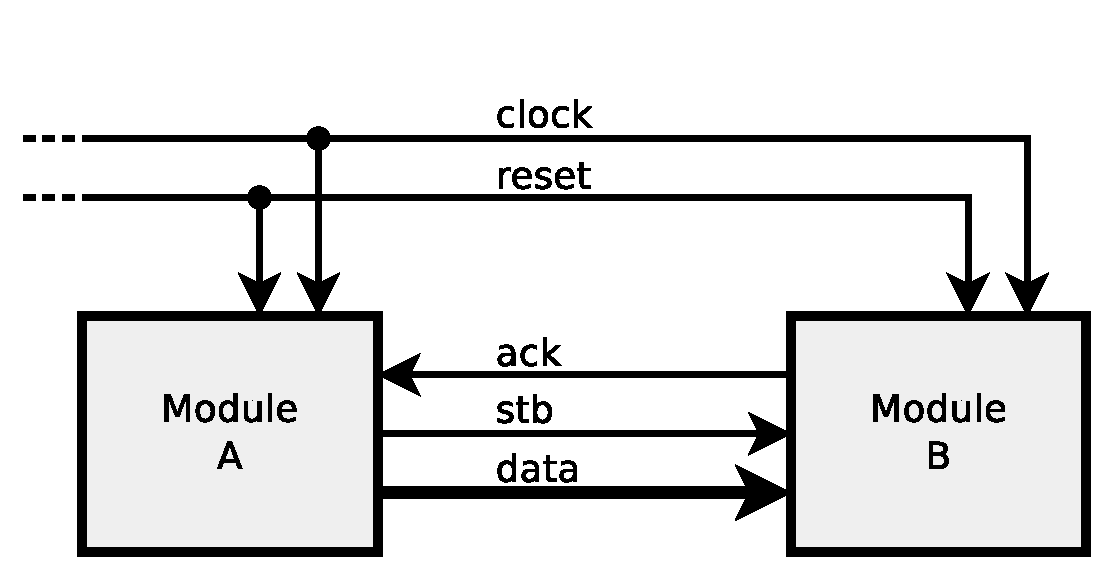
\includegraphics[width=0.4\linewidth]{digital_circ/abus.eps}
    \caption{Synchronous Interconnect Bus Diagram}
    \label{fig:abus}
\end{figure}
        
Due to these reasons, further neural network development in HDL will wait until Oliver finalises better arithmetic operation modules.
